\chapter{NDT SLAM problem analysis}

Solving full \gls{SLAM} problems requires combining algorithms for position estimation, mapping and measurement data registration. 
Solution to mapping and localization starts with initial data from sensors. Every solution to full SLAM requires different input data. Standard is to expect odometry information about relative movement of robot and some measurements of environment for map building. \gls{SLAM} problems were first studied with only sonar measurement and odometry from wheel encoders. Sonars were later replaced by more sophisticated laser scanners. An odometry got more exact with use of \gls{IMU}. Alternatively, full \gls{SLAM} problem is also solved with use of camera images for both odometry and map building. Visual methods are very popular mostly in 3D mapping of environment. 

Types of \gls{SLAM}s based on lasers is still wildly used in real life applications. More research was done in 2D variant. It is generally less computationally expensive to perform 2D \gls{SLAM}. This is mostly because full solution needs to include data registration process. It is used for variety of tasks e.g., map building, odometry estimation, unique feature detection.... Some techniques used in registration are described in section \ref{Scan_reg}.

Every solution also needs to output some type of map, which should be used for navigation and planning of robot. Every solution again uses different mapping technique. The map can be represented as a set of unique landmarks or as a set of measurements integrated together. Some of these integration methods are presented in section \ref{MAP_REPRE}

Lastly we need to estimate position of robot based on our data and created map. First we need to define what it is position of robot and how we will represent it.   
\section{SLAM problem definition}
\label{sec:SLAM_def}
Successfully solving \gls{SLAM} problem means to find location of robot in every time step and be able to create map at that time-stamp. In real world we deal with robot's sensors which have always some inherited noise. This means we are not able to fully say exact position of robot. This is main reason why to use probabilistic definition of problem. Robot moves through unknown space along trajectory expressed as variables $ \textbf{x}_{1:T} = \{\textbf{x}_{1},...,\textbf{x}_{T}\} $. While moving robot is taking odometry measurements $ \textbf{u}_{1:T} = \{\textbf{u}_{1},...,\textbf{u}_{T}\}$ and perception of environment $ \textbf{z}_{1:T} = \{\textbf{z}_{1},...,\textbf{z}_{T}\}$ Solving SLAM than means finding out probability of the robot's trajectory $ \textbf{x}_{1:T}$ and a map \textbf{m} of local environment given all the measurements and initial pose $ \textbf{x}_{0}$:
\begin{equation}
p(\textbf{x}_{1:T}, \textbf{m}\: |\:  \textbf{z}_{1:T}, \textbf{u}_{1:T}, \textbf{x}_{0})
\end{equation}
Odometry is represented in 2D by triple $(x,y,\theta)$ or by three dimensional transformation matrix. Initial pose can be interpreted as origin of coordinate system for global map.

\section{SLAM's position estimation categories}
Over the past decade reaserch has developed three distinctive categories of \gls{SLAM} position estimation. 

First category is \gls{EKF} variant. It is based on \gls{KF}. The \gls{KF}  assume that probability density functions are Gaussian distributions and system is linear. The \gls{EKF} solves problems with non-linearity of robot pose model. Performance of \gls{EKF} strongly depends on quality of statistical model for noise in sensors and odometry. Unfortunately, these models are usually not available. A set of comparative tests for convergence and inconsistencies of \gls{EKF} is in work of \cite{EKF}.

Another category is based on \gls{PF}. Current state of the robot is represented by set of weighted particles. This brings advantage of representing uncertainty through multi-modal distributions and dealing with non-Gaussian noise. \cite{FastSlam} proposed computationally efficient method based on \gls{PF} called FastSLAM. It uses particles to represent posterior probability of motion. In addition, each particle also holds K Kallman filters representing landmark positions. It was demonstrated that it is possible to calculate high precision maps utilizing FastSLAM. Inspired by FastSlam, a method based on Rao-Blackwellized Particle Filter is proposed in \cite{Rao-PF}. Derivations of this approach are still actively used in robotics today. 

Last category is based on modeling state of the system by constructing robot's state graph and optimizing to find final robot position. In this graph nodes represent robots possible pose and edges its relative movement. Nodes may also hold information about current stae of map or laser measurements. This representation was first time used in work of \cite{LuMilios}. This technique was later improved by \cite{OlsonGS}. They have presented efficient optimization approach based on the scholastic gradient descent. It was able to correct even large graphs. Later multiple authors improved \gls{SLAM} optimization by adding hierarchies to large graphs or adding robustness to optimization process. Graph based model of SLAM offers a lot of flexibility for improvements and can be reasonably fast even on large graphs. More details about graph generation and optimization is in section \ref{sec:graph_base_slam}.

\section {Map representation}
\label{MAP_REPRE}
Successful solving SLAM problem should output map of the unknown environment. This map needs to be stored for local path planning and obstacle avoidance. It is also needed for scan registration. Algorithms for avoiding obstacles very often need precise map. Map should keep low memory consumption, because robots very often have limited access to memory. Scan registration algorithms usually might benefit from maps with high precision.

Point-cloud is map representation which stores all measured points. This is very precise representation. All input data is still in its raw form. We are not loosing any information. Scan-matching algorithms e.g. \gls{ICP} is working on top of this datastructure. It is very easy to convert from this model to different type of map if needed. Problematic is memory consumption. If robot runs for long period with higher frequency of data production, it is likely that robot will run out of memory.

Occupancy map is grid based type. It consists of grid with cells. In every cell we have just one value describing probability that this cell is occupied. Value becomes higher with more incoming data measurements. It has constant memory consumption with respect to time of robot's run-time. It is possible to use this representation for map to map registration process. This model is also possible to represent empty spaces (low probability). This feature is used by many path planning and obstacle avoidance algorithms. That is why, occupancy maps are main output format for SLAM algorithms in ROS. It is important to select good resolution of grid. Finer grid offers better detail but higher memory consumption.

Quad-tree is a tree data structure. Each node of the tree has exactly four children. Nodes are decomposing space into sub-areas. Every node has its threshold. When it is reached, cell subdivides into four smaller cells. This process dynamically change resolution of the grid. This way we get higher precision in places where it matters more. Maximal precision is usually bounded by minimal size of leaf nodes.

\gls{NDT} representation uses grid based datastructure. Each cell has normal distribution parameters calculated based on inserted points. This model offers constant memory consumption over time. In comparison, \gls{NDT} has better representation of inner points than octree (3D case of quad-tree). This was proven as convenient by \cite{Saarinen13}. They have shown that coarser \gls{NDT} grid can have similar results in precision of space representation than finer octree map. Standard \gls{NDT} representation has deeper explanation in section \ref{subsec:NDT_grid}. \gls{NDT} maps can also include information about occupancy. This extension called \gls{NDT-OM} will be presented in \ref{subsec:NDT_OM}. In addition to occupancy, this method also add a way how to remove dynamic objects from map. This is important feature if \gls{SLAM} should work in dynamic environment.      
\begin{figure}
	\centering
	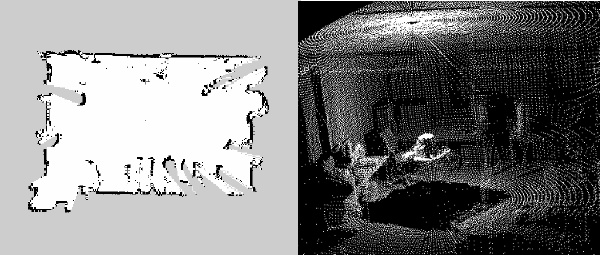
\includegraphics[width=100mm]{../img/maps.png}
	\caption{On the left is visualization of occupancy grid. On the right is visualized point cloud of a room.}
	\label{fig:maps}
\end{figure}
\newpage

\section{Registration}
\label{sec:Scan_reg}
Scan registration is one of the key concepts in full SLAM solution. Algorithm can use scan matching between two scans to determine transformation. It tells how far robot moved between scans. Two scans might not offer enough information for successful registration. Imagine a robot which is standing in the corner of a room with sensor facing the wall. Scan from this robot has only information from very limited field of view and this might lead to matching errors. Therefore, it is usually necessary to combine individual scans to operate with more data.  

One of the algorithms which uses this process is called incremental scan-matching. It takes arriving scan and tries to match it against the map built from previous measurements. By doing so it can very well be used instead of robots odometry in \gls{SLAM}'s graph creation. Algorithms which are possible to work in incremental scan-matching on top of \gls{NDT} maps are mentioned in sections \ref{subsec:P2D_NDT} and \ref{subsec:D2D_NDT}. Other often used approach is the \gls{ICP}, which is described in \ref{subsec:ICP}. All these algorithms use optimization methods, e.g. Newton's method. Good initial guess is needed in order to guarantee converge to the right solution. 

Another example of usage scan registration in graph based \gls{SLAM} is for testing generated loop closures. Loop closures are edges which close the loop (create cycle) of robot's movement in graph. Details about loop closure generation are in section \ref{subsec:loop_closure_creation}. Measurements from nodes which play role in loop closure are scan matched. By doing this we are trying to proof if two nodes are really overlapping.  The Biggest problem with this registration is that we have no valid prior information about positions of these nodes. These two scans might be perfectly aligned or they can be from completely different parts of the world. Registration needs to robustly estimate the transformation. In case of misleading closure algorithm should reject it. One scan matcher capable of robust transformation calculation is mentioned in \ref{subsec:Corr}.  

\begin{figure}
\centering
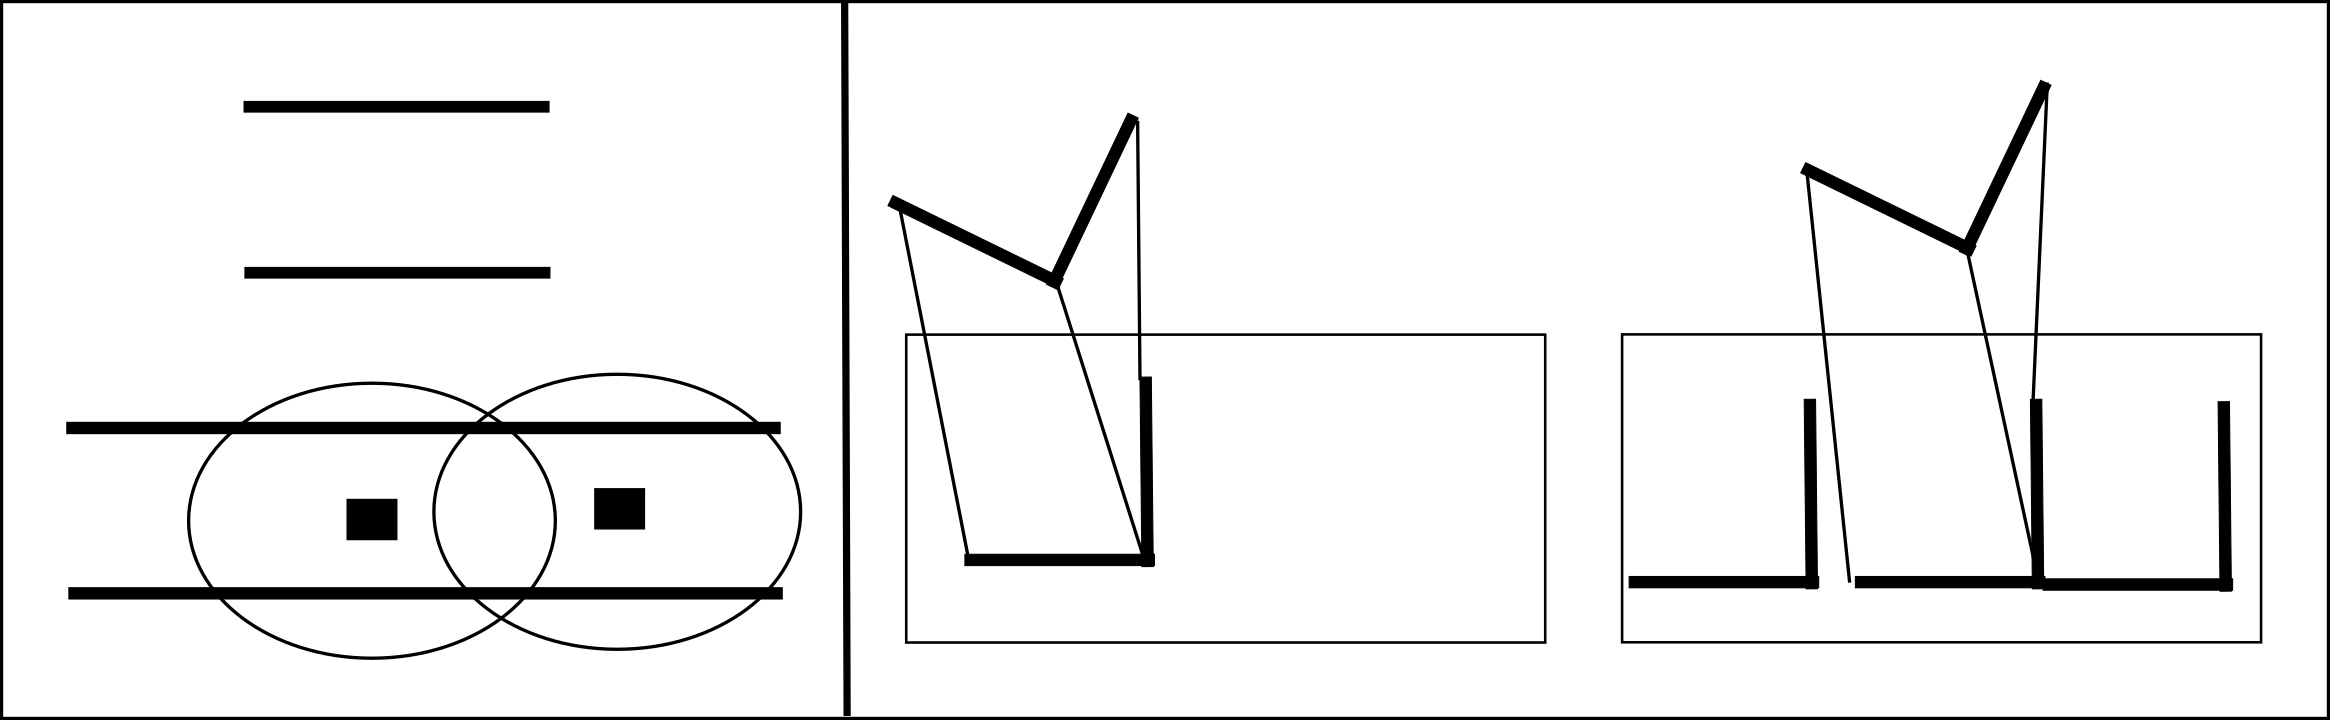
\includegraphics[width=100mm]{../img/ambi.png} 	
\caption{Local and global ambiguities in scan registrations. On the left is local ambiguity. On the right is global ambiguity with two maps. First map is original map without all information about environment. Second map is reality with all features. Registration wrongly associated matching based on information only from first map.} \label{fig:ambig}

\end{figure}

Even robust scan-matchers can fail to correctly identify loop closures.  These registration mismatches can be divided into two categories.

The First category is local ambiguity. Good example of it is when robot moves in long corridor as seen in figure \ref{fig:ambig} on the left. Environment does not have many distinctive features and algorithm selected one of three possible correct options.

The second category is global ambiguity. This ambiguity usually happens when algorithm do not have enough information about whole environment. Limited size of scans and environment with similar indistinguishable elements can resolve in wrong association. One example can be seen in figure \ref{fig:ambig} on the right.   




  
\section {Graph-based SLAM on NDT maps}


After initial research we have noticed that there is big potential in using \gls{NDT} maps for introducing full \gls{SLAM} solution. \gls{NDT} maps have good memory consumption they can hold occupancy information and reject dynamic objects with use of \gls{NDT-OM} extension \ref{subsec:NDT_OM}. Registration algorithms for alignment with initial guess on top of \gls{NDT} grids already exists. Graph based pose estimation currently represent very flexible way how to find robots position. It is also possible to extend to work on large scale maps. It also has topological information about robot movement which can be beneficial. 

Additionally, in the work of \cite{NDTOMFusion}, authors described that scan matching based on \gls{NDT} registration can provide very good result in mapping process with use of \gls{NDT-OM}. They have proven this by mapping large area with only use of global map solely created by modified method of incremental scan matching. They have noted that even though results are very accurate, there is need for solution with loop closure mechanism to improve results. In this work, they have mapped real life factory datasets with dynamic entities. \gls{NDT-OM} proven to be reliable way of removing dynamic objects and updating map.

Loop closures can be created in graph based \gls{SLAM} and additionally tested by robust scan matcher. In order to use \gls{NDT} maps this work presents robust registration method for loop closure alignment \ref{sec:Robust D2D-NDT}. 

It was also necessary to find solution how to represent the map. In previous works there was always one global \gls{NDT} map. Iterative scan matching than used this map for more precise alignment. In our work we use graph pose estimation which is making changes to the based on graph optimization. We present a way how to represent the map which can be updated \ref{sec:NDT_frame}.

Incremental scan matching on \gls{NDT} grids was proven to get good results. Therefore, it should be included in this work as well and combine it with rest of proposed system \ref{sec:window}.   

Lastly, it needs to be implemented in a way that on-line processing of real datasets is possible. It needs to have standard \gls{ROS} interface commonly found in other \gls{SLAM}. It should use standard libraries available in \gls{ROS}.

Final result of this works should be implementation of 2D graph based \gls{SLAM} on \gls{NDT} maps with easy use inside of \gls{ROS} ecosystem. 